\begin{figure}[ht]
    \centering
    % Subfigure 1
    \begin{subfigure}{0.32\textwidth}
        \centering
        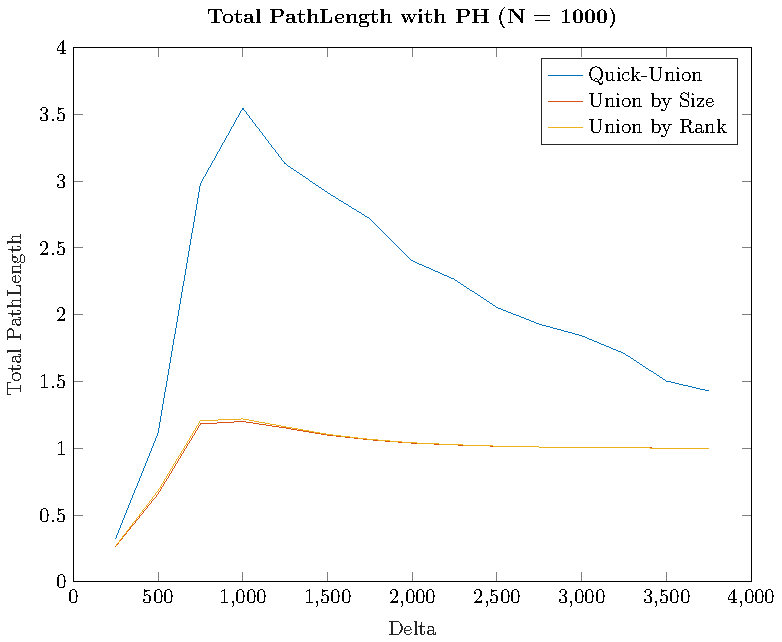
\includegraphics[width=\textwidth]{../images/plotPHFull1000_PathLength.pdf}
        \caption{Path Lengths with different union strategies with $n = 1000$}
    \end{subfigure}%
    \hfill
    % Subfigure 2
    \begin{subfigure}{0.32\textwidth}
        \centering
        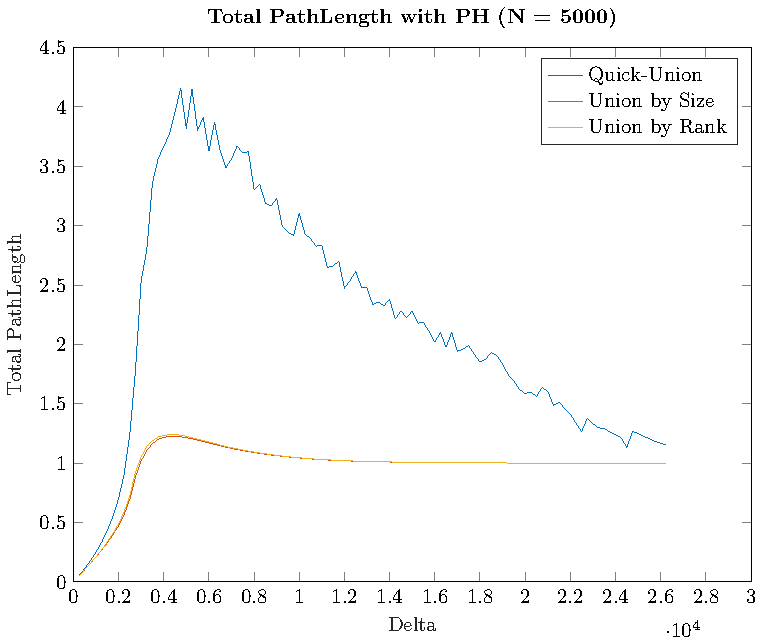
\includegraphics[width=\textwidth]{../images/plotPHFull5000_PathLength.pdf}
        \caption{Path Lengths with different union strategies with $n = 5000$}
    \end{subfigure}%
    \hfill
    % Subfigure 3
    \begin{subfigure}{0.32\textwidth}
        \centering
        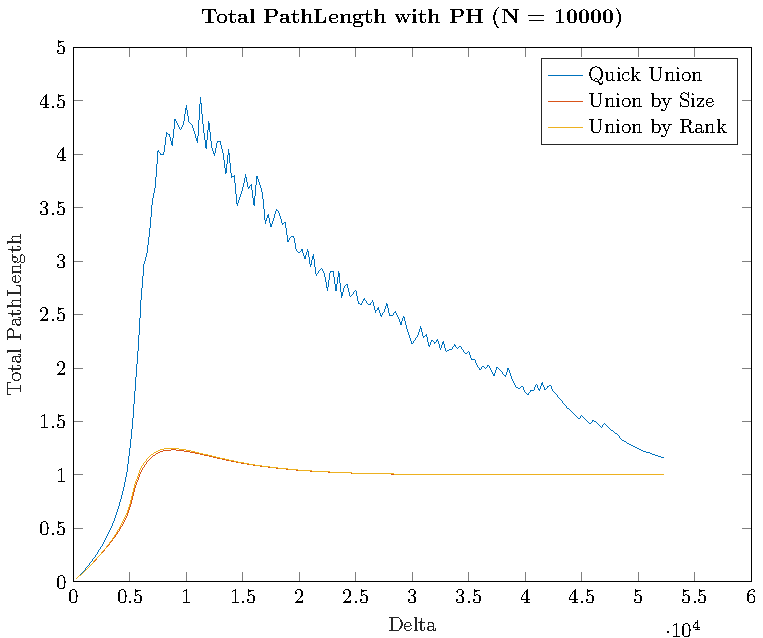
\includegraphics[width=\textwidth]{../images/plotPHFull10000_PathLength.pdf}
        \caption{Path Lengths with different union strategies with $n = 10000$}
    \end{subfigure}

    \caption{Total Path Length normalized with Path Halving}
    \label{fig:tplPH}
\end{figure}

\begin{figure}[ht]
    \centering
    % Subfigure 1
    \begin{subfigure}{0.32\textwidth}
        \centering
        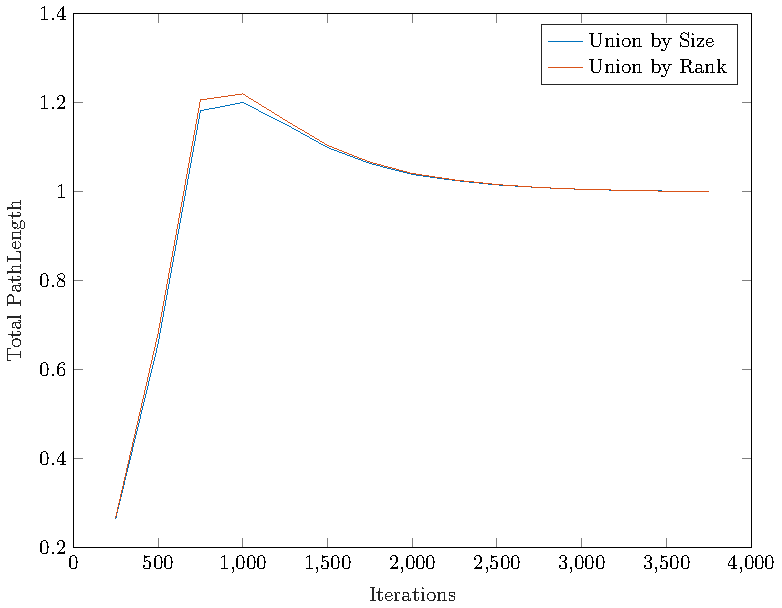
\includegraphics[width=\textwidth]{../images/plotPHNonFull1000_PathLength.pdf}
        \caption{Path Lengths with different union strategies with $n = 1000$}
    \end{subfigure}%
    \hfill
    % Subfigure 2
    \begin{subfigure}{0.32\textwidth}
        \centering
        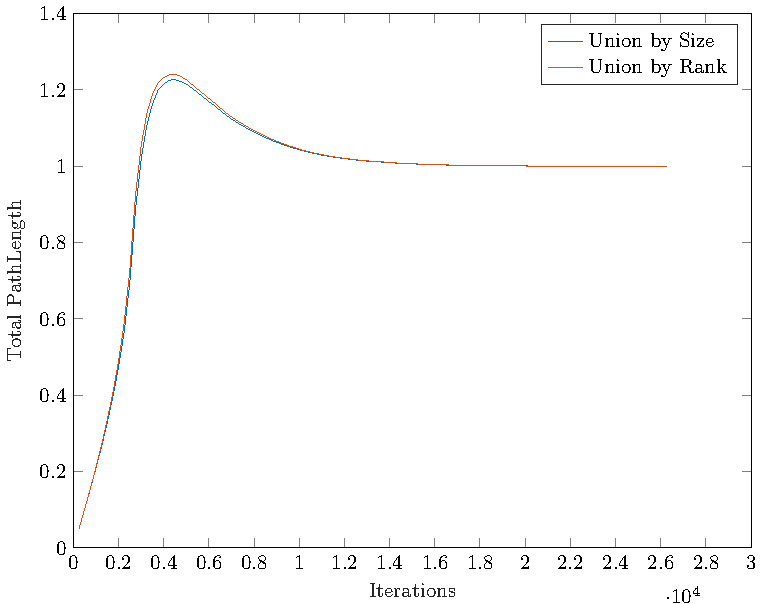
\includegraphics[width=\textwidth]{../images/plotPHNonFull5000_PathLength.pdf}
        \caption{Path Lengths with different union strategies with $n = 5000$}
    \end{subfigure}%
    \hfill
    % Subfigure 3
    \begin{subfigure}{0.32\textwidth}
        \centering
        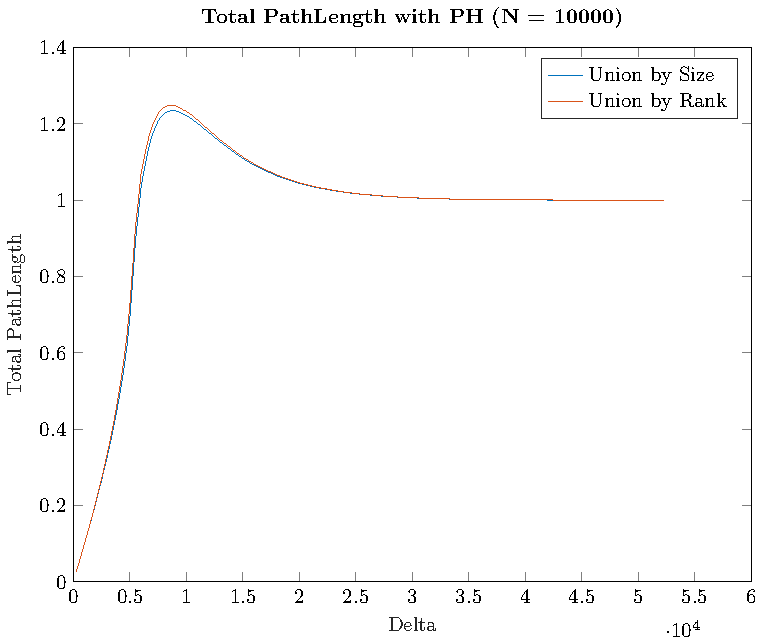
\includegraphics[width=\textwidth]{../images/plotPHNonFull10000_PathLength.pdf}
        \caption{Path Lengths with different union strategies with $n = 10000$}
    \end{subfigure}

    \caption{Total Path Length normalized with Path Halving without Quick-Union}
    \label{fig:tplPHNoQU}
\end{figure}


\begin{figure}[ht]
    \centering
    % Subfigure 1
    \begin{subfigure}{0.32\textwidth}
        \centering
        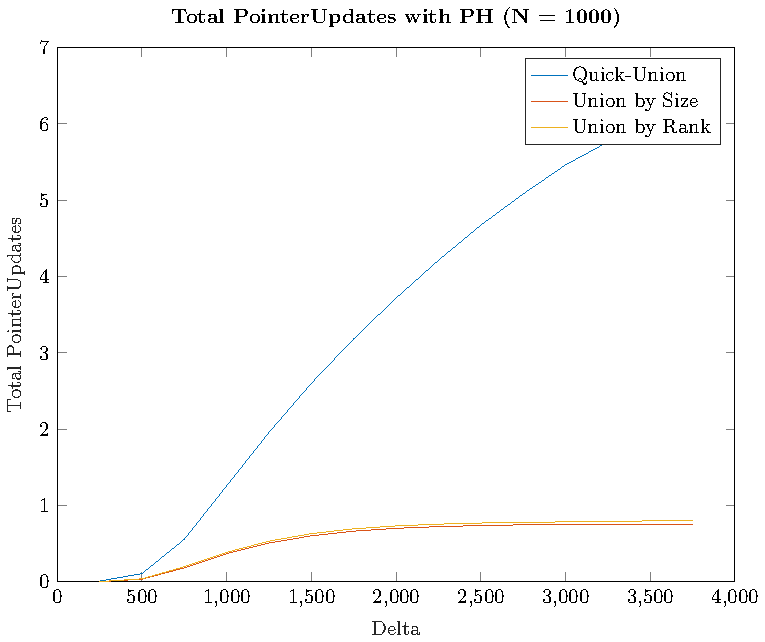
\includegraphics[width=\textwidth]{../images/plotPHFull1000_PointerUpdates.pdf}
        \caption{Pointer Updates with different union strategies with $n = 1000$}
    \end{subfigure}%
    \hfill
    % Subfigure 2
    \begin{subfigure}{0.32\textwidth}
        \centering
        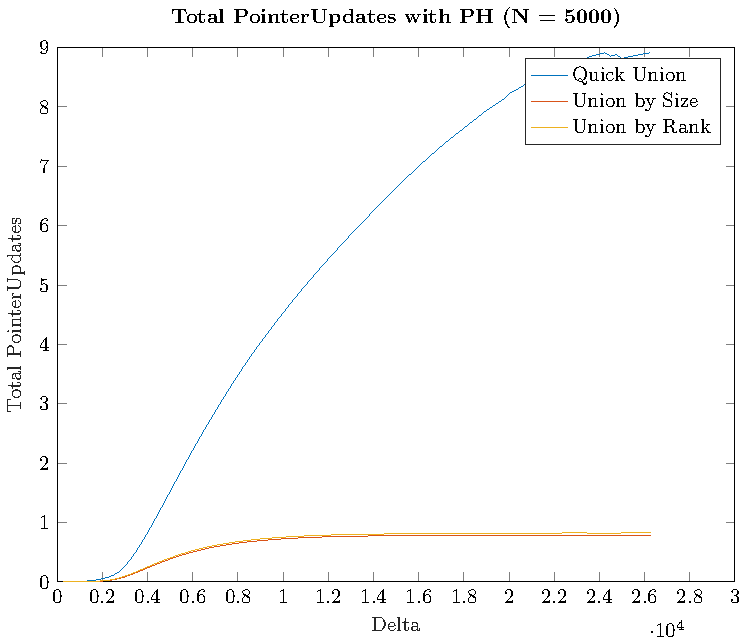
\includegraphics[width=\textwidth]{../images/plotPHFull5000_PointerUpdates.pdf}
        \caption{Pointer Updates with different union strategies with $n = 5000$}
    \end{subfigure}%
    \hfill
    % Subfigure 3
    \begin{subfigure}{0.32\textwidth}
        \centering
        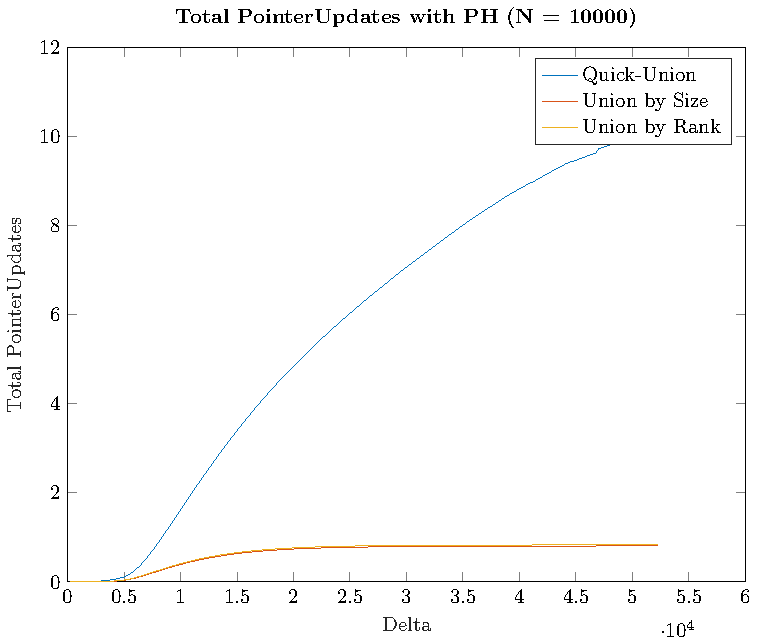
\includegraphics[width=\textwidth]{../images/plotPHFull10000_PointerUpdates.pdf}
        \caption{Pointer Updates with different union strategies with $n = 10000$}
    \end{subfigure}

    \caption{Total Pointer Update normalized with Path Halving}
    \label{fig:tpuPH}
\end{figure}


\begin{figure}[ht]
    \centering
    % Subfigure 1
    \begin{subfigure}{0.32\textwidth}
        \centering
        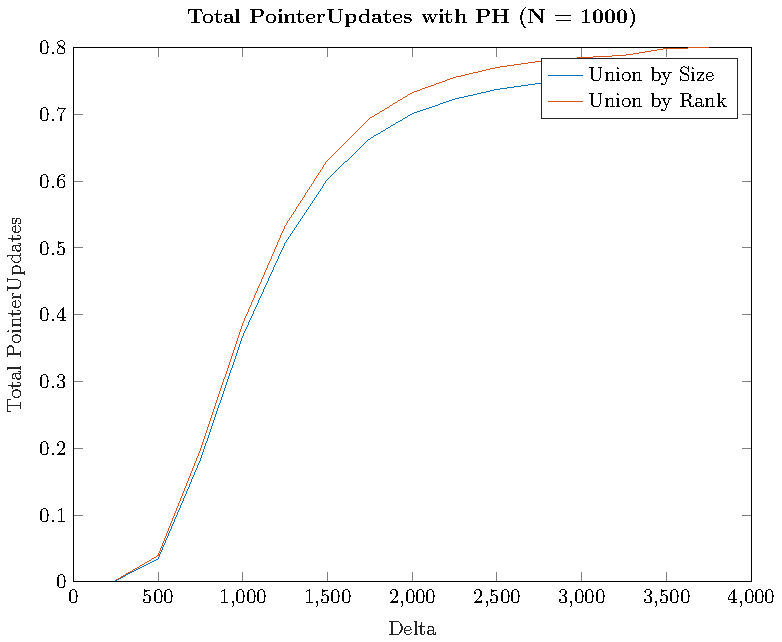
\includegraphics[width=\textwidth]{../images/plotPHNonFull1000_PointerUpdates.pdf}
        \caption{Pointer Updates with different union strategies with $n = 1000$}
    \end{subfigure}%
    \hfill
    % Subfigure 2
    \begin{subfigure}{0.32\textwidth}
        \centering
        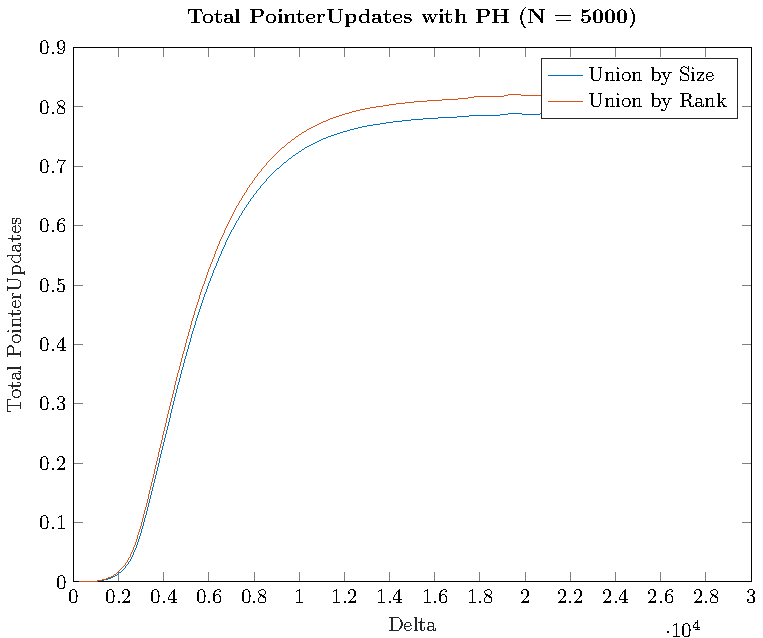
\includegraphics[width=\textwidth]{../images/plotPHNonFull5000_PointerUpdates.pdf}
        \caption{Pointer Updates with different union strategies with $n = 5000$}
    \end{subfigure}%
    \hfill
    % Subfigure 3
    \begin{subfigure}{0.32\textwidth}
        \centering
        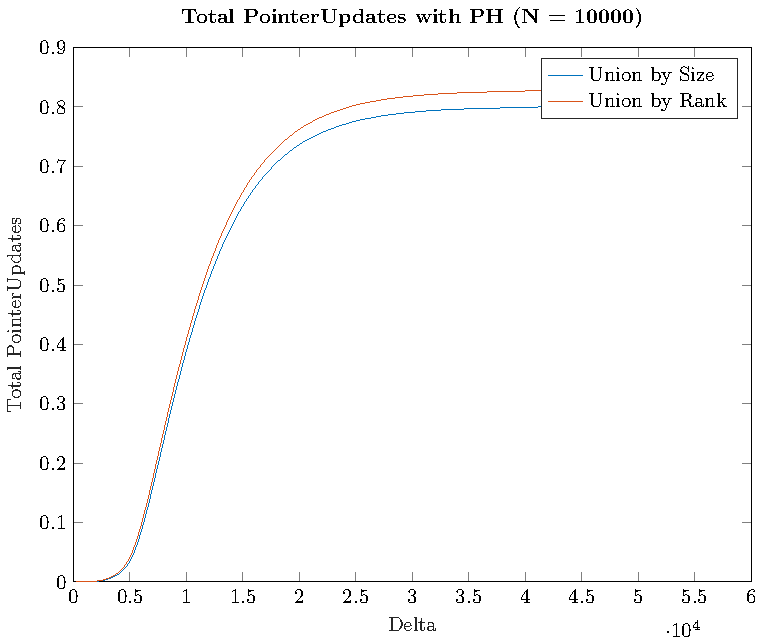
\includegraphics[width=\textwidth]{../images/plotPHNonFull10000_PointerUpdates.pdf}
        \caption{Pointer Updates with different union strategies with $n = 10000$}
    \end{subfigure}

    \caption{Total Pointer Update normalized with Path Halving without Quick-Union}
    \label{fig:tpuPHNoQU}
\end{figure}
